\documentclass[runningheads]{../llncs}

\usepackage{tabularx}
\usepackage{booktabs}
\usepackage[export]{adjustbox}
\usepackage{array}
\newcolumntype{L}[1]{>{\raggedright\let\newline\\\arraybackslash\hspace{0pt}}p{#1}}
\newcolumntype{C}[1]{>{\centering\let\newline\\\arraybackslash\hspace{0pt}}p{#1}}
\newcolumntype{R}[1]{>{\raggedleft\let\newline\\\arraybackslash\hspace{0pt}}p{#1}}

% Used for displaying a sample figure. If possible, figure files should
% be included in EPS format.
\usepackage{graphicx}
\graphicspath{{../images/}}

% If you use the hyperref package, please uncomment the following line
% to display URLs in blue roman font according to Springer's eBook style:
\usepackage[colorlinks=true, linkcolor=blue, urlcolor=blue, citecolor=blue, anchorcolor=blue]{hyperref}
\renewcommand\UrlFont{\rmfamily}

\begin{document}

\title{Learning Grasp Evaluation Models Using Synthetic 3D Object-Grasp Representations}

%\titlerunning{Abbreviated paper title}
% If the paper title is too long for the running head, you can set
% an abbreviated paper title here
%
\author{
    Minh Nguyen \inst{1} \and
    Paul G. Pl\"{o}ger \and
    Alex Mitrevski\inst{1} \and
    Maximilian Sch\"{o}bel\inst{1}}
%
\authorrunning{M. Nguyen et al.}
% First names are abbreviated in the running head.
% If there are more than two authors, 'et al.' is used.
%
\institute{Hochschule Bonn-Rhein-Sieg, Grantham-Allee 20, 53757 Sank Augustin, Germany \\
\email{minh.nguyen@smail.h-brs.de}, \email{\{paul.ploeger,aleksandar.mitrevski,maximilian.schoebel\}@h-brs.de}}
%
\maketitle              % typeset the header of the contribution

\begin{abstract}
This project considers the problem of generating data for training grasp evaluation models. Recent advances are reviewed
for four main aspects most relevant to labeled grasp data synthesis, namely feature extraction from perceptual data,
object-grasp representation, grasp evaluation techniques, and data generation techniques. From this review, one may
conclude that while data synthesis for learning a grasp evaluation model is promising, recent approaches are either
limited by difficulties in collecting large-scale human grasp experience, or by the shortcomings of using analytical
metrics to label generated data. Additionally, a completed object grasping pipeline is integrated, from object
detection to grasp pose detection and grasp execution. Two set of experiments are performed on the Toyota Human Support
Robot for two pose estimation methods using this grasping pipeline. The pipeline proves reliable and fast enough for
performing the experiments, being able to execute 20 grasps per object without interruption. While further extension and
optimization are needed, the pipeline enables directly examining and comparing more advanced grasp planning methods in
the future.

\keywords{Grasp learning \and Data synthesis.}
\end{abstract}


\section{Introduction}

\subsection{Motivation}

Robot grasping with multi-fingered robotic hands is a challenging problem, and finding a grasp planning solution which
resembles humans' grasps in dexterity and robustness is still an area of active research.

\subsection{Use Case}

\begin{itemize}
    \item This project focuses on grasping tasks relevant to the Robocup@Home
            \footnote{\url{http://www.robocupathome.org}} competition. These tasks involve objects which can be commonly
            found in a domestic environment, some of which can be seen in figure \ref{fig:robocup_objects}.
    \item The experiments will be conducted on the Human Support Robot (HSR) from Toyota
            \footnote{\url{https://www.toyota-global.com/innovation/partner_robot/robot/}}.
\end{itemize}

\begin{figure}[h!]
    \centering
    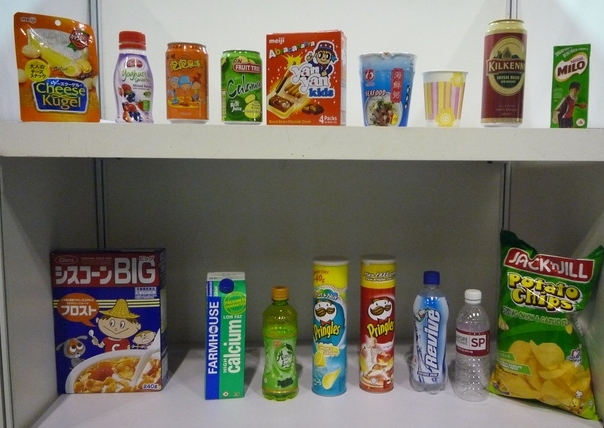
\includegraphics[width=0.6\textwidth]{robocup_typical_objects}
    \caption{Typical objects in the Robocup@Home competition \cite{robocupRulebook2018}.}
    \label{fig:robocup_objects}
\end{figure}

\subsection{Overview of robotic grasping research}

\section{State of the Art}

\begin{table}[h!]
    \scriptsize
    \def\arraystretch{1.2}
    \begin{tabularx}{\linewidth}{L{0.05\linewidth}C{0.39\linewidth}L{0.28\linewidth}L{0.28\linewidth}}
        Method & Object-grasp\linebreak representation & Feature extraction \& learning model & Data generation \\
        \toprule
        \cite{jiang2011}    & 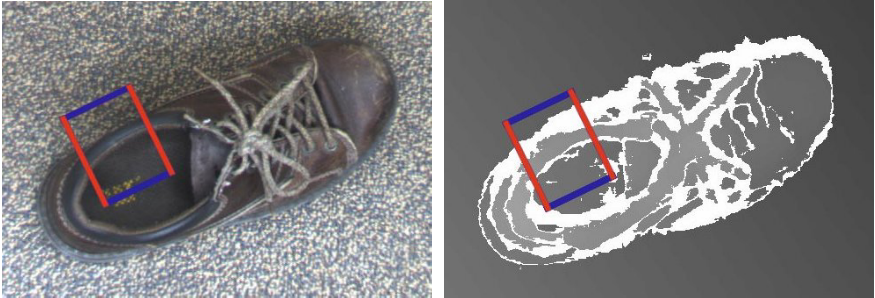
\includegraphics[scale=0.09,valign=t]{jiang_et_al-2011-grasp_representation}
        & Histogram of hand-crafted filters; \linebreak Model: SVM.
        & Rectangles manually \linebreak annotated. \\
        \cite{lenz2015}     & 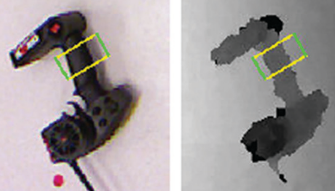
\includegraphics[scale=0.16,valign=t]{lenz_et_al-2015-grasp_representation}
        & Auto-encoders to initialize weights, structured regularization to combine depth
        and RGB data; \linebreak Model: MLP.
        & Extension of the \linebreak dataset from \cite{jiang2011} \linebreak (above).\\
        \cite{Kappler2015}  &
        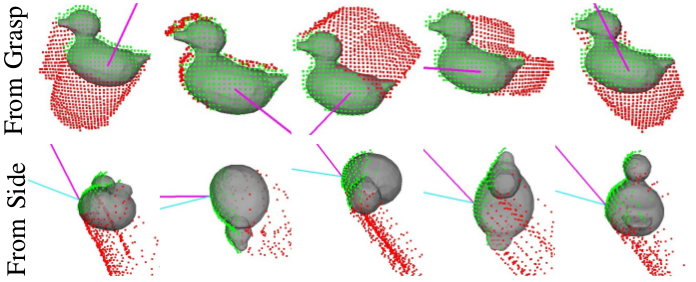
\includegraphics[scale=0.16,valign=t]{kappler_et_al-2015-fig8-local_shape_diff_viewpoints}
        & RGB rendering of ``template grids''; \linebreak Model: LeNet CNN
        & Quality of grasps are \linebreak calculated in simulation \linebreak for object
        meshes, \linebreak verified via crow-sourcing. \\
        \cite{Gualtieri2016}& 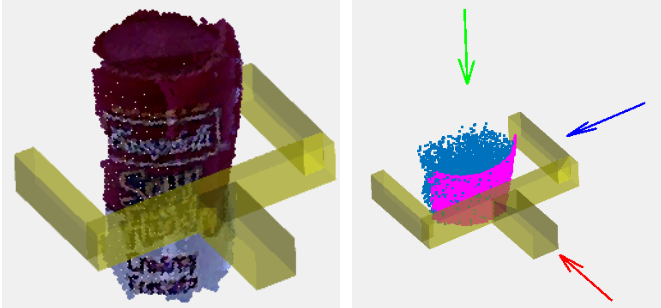
\includegraphics[scale=0.1,valign=t]{Gualtieri_et_al-2016-grasp_representation}
        & Filters of cuboid regions projected onto 3 orthogonal planes, creating 15 channels;
        \linebreak Model: LeNet CNN.
        & Quality of grasps are \linebreak calculated for object \linebreak meshes using
        force-closure \\
        \cite{mahler2017}   & 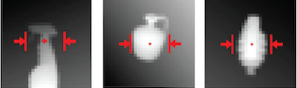
\includegraphics[scale=0.22,valign=t]{mahler_et_al-2017-grasp_representation}
        & Depth images cropped and aligned to gripper; \linebreak Model: CNN combined
        with single-layer NN.
        & Quality of grasps are \linebreak calculated for object \linebreak meshes using a
        variant of $ \epsilon $-metric from \cite{WeiszAllen2012} \\
        \bottomrule
    \end{tabularx}
    \caption{\scriptsize Five recent empirical approaches to grasp quality prediction}
    \label{table:grasp_approaches}
\end{table}

\section{Methodology}

\section{Experiments}

\section{Conclusion}

The first contribution of this work is a detailed review of recent advances in aspects most relevant to generating data
for training a grasp evaluation models, namely feature extraction from perceptual data, object-grasp representation,
grasp evaluation metrics, and data generation techniques. Additionally, five recent, prominent approaches to data
synthesis for grasp evaluation are examined, and their solutions for each of the four aspects mentioned above are
summarized in table \ref{table:grasp_approaches}.

The second contribution of this project is the implementation of a full grasping pipeline, from perceiving objects to
grasp execution, in collaboration with another Research and Development project by Padalkar \cite{Padalkar2018}. Two
pose estimation methods are implemented, serving as baselines for experimenting and comparing with more advanced grasp
planning techniques.

The review of recent approaches to grasp data synthesis demonstrates their limitations either in dataset size or by
using theoretical approaches to generate data labels, suggesting possible extensions and improvements with larger human
grasp experience database \cite{Saudabayev2018} or more advanced feature extraction methods \cite{Varley2017}.

%
\bibliographystyle{../splncs04}
\bibliography{../RnD}
%

\end{document}
